\documentclass[12pt]{article}
\usepackage{amsmath, amssymb, amsthm}
\usepackage{geometry}
\usepackage{array}
\usepackage{enumitem}
\usepackage{titlesec}
\usepackage[dvipsnames, table]{xcolor}
\usepackage{fancyhdr}
\usepackage{tcolorbox}
\usepackage[expansion=false]{microtype}
\usepackage{multicol}
\usepackage{booktabs}
\usepackage{multirow}
\usepackage{titletoc}
\usepackage{tikz}
\usetikzlibrary{arrows.meta, positioning, shapes.geometric, calc}

\tcbuselibrary{skins, breakable}

\geometry{margin=0.9in, top=1.1in, bottom=1in}
\setlength{\headheight}{16pt}

% ── Colour Palette (Deep Navy / Azure Technical Palette) ───
\definecolor{primary}  {RGB}{27,  79, 114}
\definecolor{accent}   {RGB}{46, 134, 193}
\definecolor{lightbg}  {RGB}{234, 244, 251}
\definecolor{tealclr}  {RGB}{0,  110,  90}
\definecolor{tealbg}   {RGB}{220, 245, 240}
\definecolor{amberclr} {RGB}{160, 90,   0}
\definecolor{amberbg}  {RGB}{255, 243, 220}
\definecolor{purpleclr}{RGB}{90,  20, 140}
\definecolor{purplebg} {RGB}{240, 228, 255}
\definecolor{redclr}   {RGB}{150,  20,  20}
\definecolor{redbg}    {RGB}{255, 228, 228}
\definecolor{greenclr} {RGB}{20, 120,  40}
\definecolor{greenbg}  {RGB}{220, 248, 228}
\definecolor{grayclr}  {RGB}{80,  80,  80}
\definecolor{graybg}   {RGB}{245, 245, 245}
\definecolor{darktext} {RGB}{44,  62,  80}

% ── Table of Contents styling ───────────────────────────────
\setcounter{secnumdepth}{0}
\setcounter{tocdepth}{2}
\renewcommand{\contentsname}{}
\titlecontents{section}
  [18pt]
  {\addvspace{5pt}\bfseries\color{primary}}
  {}{}
  {\color{accent!60}\titlerule*[5pt]{.}\textbf{\color{accent}\contentspage}}
\titlecontents{subsection}
  [32pt]
  {\small\color{darktext}}
  {}{}
  {\color{accent!40}\titlerule*[5pt]{.}\color{primary}\contentspage}

% ── Page style ──────────────────────────────────────────────
\pagestyle{fancy}
\fancyhf{}
\fancyhead[L]{\small\color{primary}\textbf{Differential Equations \& Modeling}\;\textcolor{accent}{|}\;System of Lake Pollution}
\fancyhead[R]{\small\color{darktext}BS Mathematics}
\renewcommand{\headrulewidth}{0pt}
\fancyhead[C]{\color{accent}\rule[-1ex]{\textwidth}{1.2pt}}
\fancyfoot[C]{\small\color{darktext}\thepage}

% ── Section styling ─────────────────────────────────────────
\titleformat{\section}
  {\large\bfseries\color{primary}}{}
  {0em}{}
  [\color{accent}\rule{\linewidth}{2pt}]
\titlespacing*{\section}{0pt}{16pt}{8pt}

\titleformat{\subsection}
  {\normalsize\bfseries\color{accent}}{}
  {0em}{}
\titlespacing*{\subsection}{0pt}{10pt}{4pt}

% ── Custom Environments ─────────────────────────────────────
\newtcolorbox{defbox}[1][]{
  enhanced, arc=4pt, boxrule=1.5pt,
  colback=tealbg, colframe=tealclr,
  left=10pt, right=10pt, top=8pt, bottom=8pt,
  title={\small\bfseries\color{white} Definition\ifx&#1&\else\ ---\ #1\fi},
  colbacktitle=tealclr, coltitle=white,
  attach boxed title to top left={xshift=10pt, yshift=-\tcboxedtitleheight/2},
  boxed title style={arc=3pt, colframe=tealclr, boxrule=0pt},
}

\newtcolorbox{thmbox}[1][]{
  enhanced, arc=4pt, boxrule=1.5pt,
  colback=amberbg, colframe=amberclr,
  left=10pt, right=10pt, top=8pt, bottom=8pt,
  title={\small\bfseries\color{white} Mathematical Law / Theorem\ifx&#1&\else\ ---\ #1\fi},
  colbacktitle=amberclr, coltitle=white,
  attach boxed title to top left={xshift=10pt, yshift=-\tcboxedtitleheight/2},
  boxed title style={arc=3pt, colframe=amberclr, boxrule=0pt},
}

\newtcolorbox{derivbox}[1][]{
  enhanced, arc=4pt, boxrule=1.5pt,
  colback=lightbg, colframe=primary,
  left=10pt, right=10pt, top=8pt, bottom=8pt,
  title={\small\bfseries\color{white} Derivation \& Formulation\ifx&#1&\else\ ---\ #1\fi},
  colbacktitle=primary, coltitle=white,
  attach boxed title to top left={xshift=10pt, yshift=-\tcboxedtitleheight/2},
  boxed title style={arc=3pt, colframe=primary, boxrule=0pt},
}

\newtcolorbox{formulabox}{
  enhanced, arc=4pt, boxrule=1.5pt,
  colback=lightbg, colframe=accent,
  left=10pt, right=10pt, top=8pt, bottom=8pt,
  title={\small\bfseries\color{white} Key Governing Equation},
  colbacktitle=accent, coltitle=white,
  attach boxed title to top left={xshift=10pt, yshift=-\tcboxedtitleheight/2},
  boxed title style={arc=3pt, colframe=accent, boxrule=0pt},
}

\newtcolorbox{examplebox*}[1][]{
  enhanced, breakable,
  colback=white, colframe=amberclr, arc=5pt, boxrule=1.5pt,
  left=12pt, right=12pt, top=8pt, bottom=8pt,
  title={\small\bfseries\color{white} Worked Example\ifx&#1&\else\ ---\ #1\fi},
  colbacktitle=amberclr, coltitle=white,
  attach boxed title to top left={xshift=10pt, yshift=-\tcboxedtitleheight/2},
  boxed title style={arc=3pt, colframe=amberclr, boxrule=0pt},
}

\newtcolorbox{keybox}[1][]{
  enhanced,
  borderline west={4pt}{0pt}{purpleclr},
  colback=purplebg!60, colframe=white,
  arc=0pt, boxrule=0pt,
  left=12pt, right=8pt, top=6pt, bottom=6pt,
}

\newtcolorbox{notebox}{
  enhanced,
  borderline west={4pt}{0pt}{redclr},
  colback=redbg!60, colframe=white,
  arc=0pt, boxrule=0pt,
  left=12pt, right=8pt, top=6pt, bottom=6pt,
}

\newcolumntype{C}[1]{>{\centering\arraybackslash}p{#1}}
\newcommand{\hcell}[1]{\textbf{\color{white}#1}}

\begin{document}

% ════════════════════════════════════════════════════════════
%  COVER PAGE
% ════════════════════════════════════════════════════════════
\thispagestyle{empty}

\begin{tcolorbox}[
  enhanced, arc=0pt, boxrule=0pt,
  colback=primary, colframe=primary,
  left=20pt, right=20pt, top=26pt, bottom=20pt,
  borderline south={5pt}{0pt}{accent},
]
  \centering
  {\fontsize{24}{30}\bfseries\color{white}
    System of Lake Pollution\\[8pt]
    Mathematical Modeling \& Analytical Solutions
  }\\[12pt]
  {\large\color{lightbg}
    Coupled ODE Systems \textbf{·} Compartmental Analysis \textbf{·} Matrix Exponential \textbf{·} Clean-Up Dynamics
  }
\end{tcolorbox}

\vspace{8pt}

\begin{tcolorbox}[
  enhanced, arc=0pt, boxrule=0pt,
  colback=white, colframe=white,
  borderline north={2pt}{0pt}{primary},
  borderline south={2pt}{0pt}{primary},
  left=0pt, right=0pt, top=0pt, bottom=0pt,
]
\begin{tabular}{p{0.32\textwidth} | p{0.34\textwidth} | p{0.28\textwidth}}
  \hspace{10pt}\begin{minipage}[t]{0.30\textwidth}\vspace{8pt}
    {\footnotesize\bfseries\color{accent} TEACHER}\\[4pt]
    {\bfseries\color{primary} Dr.\ Inayatullah}\\[3pt]
    {\footnotesize\color{darktext} Dept.\ of Mathematics}
  \vspace{8pt}\end{minipage}
  &
  \hspace{10pt}\begin{minipage}[t]{0.32\textwidth}\vspace{8pt}
    {\footnotesize\bfseries\color{accent} COMPOSED BY}\\[4pt]
    {\bfseries\color{primary} Nadir Ali Khan}\\[3pt]
    {\footnotesize\color{darktext} Roll No: MT-0123-052}
  \vspace{8pt}\end{minipage}
  &
  \hspace{10pt}\begin{minipage}[t]{0.26\textwidth}\vspace{8pt}
    {\footnotesize\bfseries\color{accent} INSTITUTION}\\[4pt]
    {\bfseries\color{primary} SALU Khairpur}\\[3pt]
    {\footnotesize\color{darktext} BS-IV Mathematics}
  \vspace{8pt}\end{minipage}
\end{tabular}
\end{tcolorbox}

\vspace{10pt}

% Table of Contents Card
\begin{tcolorbox}[
  enhanced, arc=4pt, boxrule=1.5pt,
  colback=white, colframe=primary,
  left=16pt, right=16pt, top=10pt, bottom=10pt,
  title={\bfseries\color{white}\large Contents \& Module Structure},
  colbacktitle=primary, coltitle=white,
]
  \tableofcontents
\end{tcolorbox}

\newpage

% ════════════════════════════════════════════════════════════
%  SECTION 1: PHYSICAL FORMULATION & CONSERVATION LAW
% ════════════════════════════════════════════════════════════
\section{1. Physical Description \& Compartmental Principle}

The \textbf{System of Lake Pollution} is a classical application of first-order coupled linear ordinary differential equations. It models how contaminants (such as industrial effluent, pesticides, or heavy metals) disperse, mix, and wash out through a network of interconnected lakes, channels, and reservoirs (notably inspired by the Laurentian Great Lakes system).

\begin{defbox}[Well-Mixed Lake Compartment]
Let $V_i$ denote the constant volume of Lake $i$ (in $\text{m}^3$ or $\text{km}^3$), and let $x_i(t)$ represent the total mass of pollutant present in Lake $i$ at time $t$ (in $\text{kg}$ or $\text{metric tons}$).
The uniform concentration of pollutant $c_i(t)$ throughout Lake $i$ is:
\begin{equation}
  c_i(t) = \frac{x_i(t)}{V_i} \quad \left[\text{mass} / \text{volume}\right].
\end{equation}
The well-mixed hypothesis assumes that the pollutant disperses instantaneously and homogeneously throughout the entire lake volume.
\end{defbox}

\begin{thmbox}[Conservation of Pollutant Mass]
For any lake compartment $i$, the time rate of change of total pollutant mass equals the rate at which pollutant enters minus the rate at which pollutant leaves:
\begin{equation}
  \frac{dx_i}{dt} = \text{Rate}_{\text{in}} - \text{Rate}_{\text{out}}.
\end{equation}
If water flows into Lake $i$ from Lake $j$ at volumetric flow rate $F_{ji}$ with concentration $c_j(t)$, and clean/polluted water enters from an external source at rate $F_{\text{ext}, i}$ with concentration $c_{\text{ext}, i}(t)$, then:
\begin{equation}
  \text{Rate}_{\text{in}} = \sum_{j \neq i} F_{ji} \frac{x_j(t)}{V_j} + F_{\text{ext}, i} c_{\text{ext}, i}(t).
\end{equation}
Similarly, if water flows out of Lake $i$ at total outflow rate $F_{\text{out}, i}$, the mass outflow rate is:
\begin{equation}
  \text{Rate}_{\text{out}} = F_{\text{out}, i} c_i(t) = \frac{F_{\text{out}, i}}{V_i} x_i(t).
\end{equation}
\end{thmbox}

\begin{keybox}
\textbf{Hydrodynamic Equilibrium (Constant Volume):}\\
To maintain constant lake volumes, the total volumetric water inflow must equal the total volumetric outflow for each lake:
\[
  \sum_{\text{in}} F = \sum_{\text{out}} F \implies \frac{dV_i}{dt} = 0.
\]
The ratio $k_i = \dfrac{F_{\text{out}, i}}{V_i}$ has dimensions of $[1/\text{time}]$ and represents the \textbf{turnover rate} (reciprocal of the mean residence time $\tau_i = V_i / F_{\text{out}, i}$).
\end{keybox}

\vspace{8pt}

% ── Network Topology Diagram ─────────────────────────────────
\begin{center}
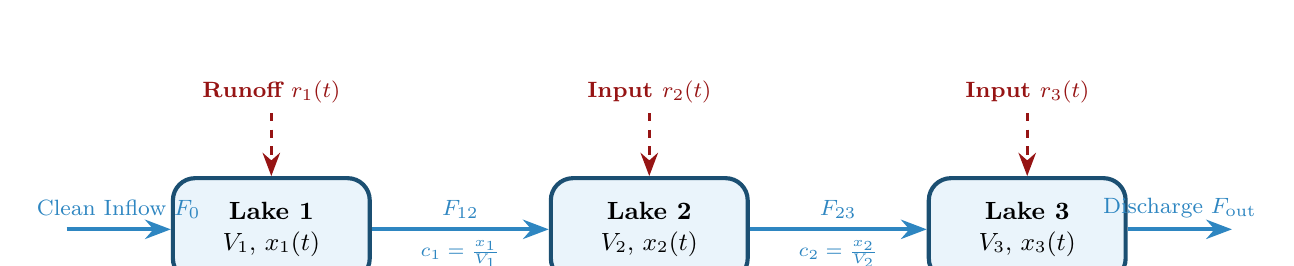
\begin{tikzpicture}[>=Stealth,
  lake/.style={draw=primary, line width=1.5pt, rounded corners=8pt, fill=lightbg, minimum width=2.5cm, minimum height=1.3cm, align=center, font=\small\bfseries},
  pipe/.style={->, line width=1.4pt, color=accent},
  feed/.style={->, line width=1.2pt, color=redclr, dashed}
]
  % Nodes
  \node[lake] (L1) at (0,0) {Lake 1\\$V_1,\, x_1(t)$};
  \node[lake] (L2) at (4.8,0) {Lake 2\\$V_2,\, x_2(t)$};
  \node[lake] (L3) at (9.6,0) {Lake 3\\$V_3,\, x_3(t)$};

  % External Inputs
  \node[above=0.8cm of L1, color=redclr, font=\footnotesize\bfseries] (in1) {Runoff $r_1(t)$};
  \node[above=0.8cm of L2, color=redclr, font=\footnotesize\bfseries] (in2) {Input $r_2(t)$};
  \node[above=0.8cm of L3, color=redclr, font=\footnotesize\bfseries] (in3) {Input $r_3(t)$};

  \draw[feed] (in1) -- (L1);
  \draw[feed] (in2) -- (L2);
  \draw[feed] (in3) -- (L3);

  % Inter-lake flows
  \draw[pipe] (-2.6,0) -- node[above, font=\footnotesize\color{darktext}] {Clean Inflow $F_0$} (L1.west);
  \draw[pipe] (L1.east) -- node[above, font=\footnotesize\color{darktext}] {$F_{12}$} node[below, font=\scriptsize\color{accent}] {$c_1 = \frac{x_1}{V_1}$} (L2.west);
  \draw[pipe] (L2.east) -- node[above, font=\footnotesize\color{darktext}] {$F_{23}$} node[below, font=\scriptsize\color{accent}] {$c_2 = \frac{x_2}{V_2}$} (L3.west);
  \draw[pipe] (L3.east) -- node[above, font=\footnotesize\color{darktext}] {Discharge $F_{\text{out}}$} (12.2,0);
\end{tikzpicture}
\end{center}

\vspace{10pt}

% ════════════════════════════════════════════════════════════
%  SECTION 2: GENERAL VECTOR-MATRIX FORMULATION
% ════════════════════════════════════════════════════════════
\section{2. Matrix State-Space Representation}

\begin{derivbox}[General System Formulation for $n$ Lakes]
For a network of $n$ interconnected lakes, the mass of pollutant in each lake is governed by the non-homogeneous linear first-order system:
\begin{equation}
  \frac{d\mathbf{x}}{dt} = A\,\mathbf{x}(t) + \mathbf{r}(t), \quad \mathbf{x}(0) = \mathbf{x}_0,
\end{equation}
where:
\begin{itemize}[itemsep=2pt, topsep=2pt]
  \item $\mathbf{x}(t) = \begin{bmatrix} x_1(t) & x_2(t) & \cdots & x_n(t) \end{bmatrix}^T$ is the state vector of pollutant masses.
  \item $\mathbf{r}(t) = \begin{bmatrix} r_1(t) & r_2(t) & \cdots & r_n(t) \end{bmatrix}^T$ represents external contaminant influx rates ($\text{mass}/\text{time}$).
  \item $A \in \mathbb{R}^{n \times n}$ is the \textbf{transfer matrix} defined by:
  \begin{equation}
    A_{ii} = -\frac{F_{\text{out}, i}}{V_i}, \qquad A_{ij} = \frac{F_{ji}}{V_j} \quad (i \neq j).
  \end{equation}
\end{itemize}
\end{derivbox}

\begin{formulabox}
\textbf{Analytical Solution via Matrix Exponential:}\\
For constant external input vector $\mathbf{r}$ and invertible transfer matrix $A$:
\begin{equation}
  \mathbf{x}(t) = e^{At}\,\mathbf{x}_0 + A^{-1}\left(e^{At} - I\right)\mathbf{r} = e^{At}\left(\mathbf{x}_0 - \mathbf{x}^*\right) + \mathbf{x}^*,
\end{equation}
where $\mathbf{x}^* = -A^{-1}\mathbf{r}$ is the \textbf{steady-state equilibrium distribution}.
\end{formulabox}

\begin{notebox}
\textbf{Asymptotic Stability:}\\
Because each diagonal entry $A_{ii} = -\frac{F_{\text{out}, i}}{V_i} < 0$ and the sum of column entries satisfies $\sum_i A_{ij} \le 0$, by the Gershgorin Disc Theorem all eigenvalues of $A$ have strictly negative real parts:
\[
  \text{Re}(\lambda_k) < 0 \quad \forall k \in \{1, 2, \dots, n\}.
\]
Consequently, $e^{At} \to 0$ as $t \to \infty$, proving that the system is \textbf{unconditionally asymptotically stable}. Any transient perturbation dies out exponentially.
\end{notebox}

\vspace{10pt}

% ════════════════════════════════════════════════════════════
%  SECTION 3: TWO INTERCONNECTED LAKES WITH FEEDBACK
% ════════════════════════════════════════════════════════════
\section{3. Case I: Two Interconnected Lakes with Bidirectional Flow}

Consider two adjacent lakes with constant volumes $V_1$ and $V_2$. Water circulates between them:
\begin{itemize}[itemsep=2pt]
  \item Clean fresh water enters Lake 1 at rate $F_0$.
  \item Water flows from Lake 1 to Lake 2 at rate $F_{12}$.
  \item A feedback flow returns water from Lake 2 to Lake 1 at rate $F_{21}$.
  \item Outflow leaves Lake 2 into a river at rate $F_e = F_0$.
\end{itemize}

\begin{derivbox}[Flow Balance \& System Equations]
Hydrodynamic volume conservation dictates:
\[
  \text{Lake 1: } F_0 + F_{21} = F_{12}, \qquad \text{Lake 2: } F_{12} = F_{21} + F_e.
\]
The rate of change of pollutant mass in each lake is:
\begin{align}
  \frac{dx_1}{dt} &= r_1 - \frac{F_{12}}{V_1}x_1 + \frac{F_{21}}{V_2}x_2, \\
  \frac{dx_2}{dt} &= r_2 + \frac{F_{12}}{V_1}x_1 - \frac{F_{21} + F_e}{V_2}x_2.
\end{align}
In matrix notation $\dfrac{d\mathbf{x}}{dt} = A\mathbf{x} + \mathbf{r}$:
\begin{equation}
  \begin{bmatrix} \dot{x}_1 \\ \dot{x}_2 \end{bmatrix} =
  \begin{bmatrix}
    -k_1 & k_{21} \\
    k_{12} & -k_2
  \end{bmatrix}
  \begin{bmatrix} x_1 \\ x_2 \end{bmatrix} +
  \begin{bmatrix} r_1 \\ r_2 \end{bmatrix},
\end{equation}
where $k_1 = \dfrac{F_{12}}{V_1}$, $k_{21} = \dfrac{F_{21}}{V_2}$, $k_{12} = \dfrac{F_{12}}{V_1}$, and $k_2 = \dfrac{F_{21} + F_e}{V_2} = \dfrac{F_{12}}{V_2}$.
\end{derivbox}

\begin{examplebox*}[Two-Lake Numerical Problem with Complete Solution]
\textbf{Problem Statement:}\\
Two interconnected lakes have volumes $V_1 = 100 \times 10^6\,\text{m}^3$ and $V_2 = 200 \times 10^6\,\text{m}^3$. 
Water transfer rates are:
\begin{itemize}[itemsep=1pt]
  \item Fresh water input to Lake 1: $F_0 = 10 \times 10^6\,\text{m}^3/\text{year}$.
  \item Inter-lake flow from Lake 1 to Lake 2: $F_{12} = 30 \times 10^6\,\text{m}^3/\text{year}$.
  \item Return pump from Lake 2 to Lake 1: $F_{21} = 20 \times 10^6\,\text{m}^3/\text{year}$.
  \item Net discharge from Lake 2: $F_e = 10 \times 10^6\,\text{m}^3/\text{year}$.
\end{itemize}
At $t = 0$, an industrial spill introduces initial pollutant masses $x_1(0) = 500\,\text{kg}$ into Lake 1 and $x_2(0) = 0$ into Lake 2. Further pollutant input is halted ($r_1 = r_2 = 0$).
Find:
\begin{enumerate}[label=(\alph*), itemsep=1pt]
  \item The analytical equations for $x_1(t)$ and $x_2(t)$.
  \item The time $t_{\max}$ when the pollutant in Lake 2 reaches its peak value, and the maximum mass $x_2(t_{\max})$.
\end{enumerate}

\vspace{6pt}
\textbf{Step 1: Compute Rate Constants and Form Matrix $A$}\\
Using the volumes and flow rates (in units of $10^6\,\text{m}^3$):
\[
  k_1 = \frac{F_{12}}{V_1} = \frac{30}{100} = 0.3\,\text{yr}^{-1}, \quad
  k_{21} = \frac{F_{21}}{V_2} = \frac{20}{200} = 0.1\,\text{yr}^{-1},
\]
\[
  k_{12} = \frac{F_{12}}{V_1} = 0.3\,\text{yr}^{-1}, \quad
  k_2 = \frac{F_{12}}{V_2} = \frac{30}{200} = 0.15\,\text{yr}^{-1}.
\]
Thus the homogeneous system is:
\[
  \begin{bmatrix} \dot{x}_1 \\ \dot{x}_2 \end{bmatrix} =
  \begin{bmatrix} -0.3 & 0.1 \\ 0.3 & -0.15 \end{bmatrix}
  \begin{bmatrix} x_1 \\ x_2 \end{bmatrix}.
\]

\textbf{Step 2: Find the Eigenvalues and Eigenvectors}\\
The characteristic equation is $\det(A - \lambda I) = 0$:
\[
  (-0.3 - \lambda)(-0.15 - \lambda) - (0.1)(0.3) = 0
\]
\[
  \lambda^2 + 0.45\lambda + 0.045 - 0.03 = \lambda^2 + 0.45\lambda + 0.015 = 0.
\]
Factoring / Quadratic formula:
\[
  \lambda = \frac{-0.45 \pm \sqrt{0.45^2 - 4(1)(0.015)}}{2} = \frac{-0.45 \pm \sqrt{0.2025 - 0.0600}}{2} = \frac{-0.45 \pm \sqrt{0.1425}}{2}.
\]
Since $\sqrt{0.1425} \approx 0.37749$:
\[
  \lambda_1 = \frac{-0.45 + 0.37749}{2} \approx -0.03625\,\text{yr}^{-1}, \qquad
  \lambda_2 = \frac{-0.45 - 0.37749}{2} \approx -0.41375\,\text{yr}^{-1}.
\]
For eigenvector $\mathbf{v}_k = \begin{bmatrix} u_k \\ w_k \end{bmatrix}$, from the first row $(-0.3 - \lambda_k)u_k + 0.1 w_k = 0 \implies w_k = \frac{0.3 + \lambda_k}{0.1}u_k$:
\[
  \mathbf{v}_1 = \begin{bmatrix} 1 \\ \frac{0.3 - 0.03625}{0.1} \end{bmatrix} = \begin{bmatrix} 1 \\ 2.6375 \end{bmatrix}, \qquad
  \mathbf{v}_2 = \begin{bmatrix} 1 \\ \frac{0.3 - 0.41375}{0.1} \end{bmatrix} = \begin{bmatrix} 1 \\ -1.1375 \end{bmatrix}.
\]

\textbf{Step 3: Apply Initial Conditions}\\
The general solution is:
\[
  \mathbf{x}(t) = c_1 \mathbf{v}_1 e^{\lambda_1 t} + c_2 \mathbf{v}_2 e^{\lambda_2 t}.
\]
At $t = 0$, $\mathbf{x}(0) = \begin{bmatrix} 500 \\ 0 \end{bmatrix}$:
\[
  c_1 + c_2 = 500, \qquad 2.6375\,c_1 - 1.1375\,c_2 = 0.
\]
From the second equation, $c_2 = \frac{2.6375}{1.1375}c_1 \approx 2.3187\,c_1$.
Substituting into the sum:
\[
  3.3187\,c_1 = 500 \implies c_1 \approx 150.66\,\text{kg}, \quad c_2 = 500 - 150.66 = 349.34\,\text{kg}.
\]
Therefore, the pollutant profiles are:
\begin{align*}
  \mathbf{x_1(t)} &= \mathbf{150.66\,e^{-0.03625 t} + 349.34\,e^{-0.41375 t}} \quad [\text{kg}],\\
  \mathbf{x_2(t)} &= \mathbf{397.37\left(e^{-0.03625 t} - e^{-0.41375 t}\right)} \quad [\text{kg}].
\end{align*}

\textbf{Step 4: Peak Pollutant in Lake 2}\\
To find the maximum in Lake 2, set $\dfrac{dx_2}{dt} = 0$:
\[
  -0.03625\,e^{-0.03625 t} - (-0.41375)\,e^{-0.41375 t} = 0 \implies e^{(0.41375 - 0.03625)t} = \frac{0.41375}{0.03625} \approx 11.4138
\]
\[
  0.3775\,t = \ln(11.4138) \approx 2.4348 \implies \mathbf{t_{\max} \approx 6.45\,\text{years}}.
\]
The peak mass of pollutant in Lake 2 is:
\[
  x_2(6.45) = 397.37 \left(e^{-0.03625(6.45)} - e^{-0.41375(6.45)}\right) = 397.37(0.7915 - 0.0693) \approx \mathbf{287.0\,\text{kg}}.
\]
\end{examplebox*}

\vspace{10pt}

% ════════════════════════════════════════════════════════════
%  SECTION 4: THREE LAKES CASCADE (THE GREAT LAKES MODEL)
% ════════════════════════════════════════════════════════════
\section{4. Case II: The Three-Lake Cascade (Great Lakes System)}

A prominent ecological challenge is the cleanup of unilateral cascades, such as Lake Huron ($L_1$), Lake Erie ($L_2$), and Lake Ontario ($L_3$).

\begin{derivbox}[Lower-Triangular Cascade Model]
When water flows sequentially without backflow ($L_1 \to L_2 \to L_3$), the transfer matrix is \textbf{lower triangular}:
\begin{equation}
  \begin{bmatrix}
    \dot{x}_1 \\ \dot{x}_2 \\ \dot{x}_3
  \end{bmatrix} =
  \begin{bmatrix}
    -k_1 & 0 & 0 \\
    k_1 & -k_2 & 0 \\
    0 & k_2 & -k_3
  \end{bmatrix}
  \begin{bmatrix}
    x_1 \\ x_2 \\ x_3
  \end{bmatrix} +
  \begin{bmatrix}
    r_1 \\ r_2 \\ r_3
  \end{bmatrix},
\end{equation}
where $k_i = \dfrac{F}{V_i}$. The eigenvalues are precisely the diagonal entries:
\begin{equation}
  \lambda_1 = -k_1, \quad \lambda_2 = -k_2, \quad \lambda_3 = -k_3.
\end{equation}
When all $k_i$ are distinct, this can be solved sequentially via integrating factors or Laplace transforms.
\end{derivbox}

\begin{formulabox}
\textbf{Step-by-Step Explicit Cascade Solutions (Zero Input $r_i = 0$):}
\begin{align}
  x_1(t) &= x_1(0)\,e^{-k_1 t},\\
  x_2(t) &= \frac{k_1 x_1(0)}{k_2 - k_1}\left(e^{-k_1 t} - e^{-k_2 t}\right) + x_2(0)\,e^{-k_2 t},\\
  x_3(t) &= k_1 k_2 x_1(0)\left[\frac{e^{-k_1 t}}{(k_2 - k_1)(k_3 - k_1)} + \frac{e^{-k_2 t}}{(k_1 - k_2)(k_3 - k_2)} + \frac{e^{-k_3 t}}{(k_1 - k_3)(k_2 - k_3)}\right] \notag\\
  &\quad + \frac{k_2 x_2(0)}{k_3 - k_2}\left(e^{-k_2 t} - e^{-k_3 t}\right) + x_3(0)\,e^{-k_3 t}.
\end{align}
\end{formulabox}

\begin{thmbox}[Half-Life \& Cleanup Time Analysis]
If Lake $i$ is isolated and the external source is cut off, its cleanup dynamics follow exponential decay:
\begin{equation}
  x_i(t) = x_i(0) e^{-k_i t}.
\end{equation}
\begin{itemize}[itemsep=3pt]
  \item \textbf{Half-Life ($t_{1/2}$):} Time required to purge $50\%$ of pollutant:
  \[
    t_{1/2} = \frac{\ln 2}{k_i} = \tau_i \ln 2 \approx 0.693\,\tau_i.
  \]
  \item \textbf{$95\%$ Purge Time ($t_{0.05}$):} Time required to remove $95\%$ of pollutant:
  \[
    t_{0.05} = \frac{\ln(1/0.05)}{k_i} = \frac{\ln 20}{k_i} \approx 2.996\,\tau_i \approx 3\,\tau_i.
  \]
  \item \textbf{$99\%$ Purge Time ($t_{0.01}$):}
  \[
    t_{0.01} = \frac{\ln(100)}{k_i} \approx 4.605\,\tau_i.
  \]
\end{itemize}
\end{thmbox}

\vspace{10pt}

% ════════════════════════════════════════════════════════════
%  SECTION 5: STEADY-STATE ANALYSIS & POLLUTION ABATEMENT
% ════════════════════════════════════════════════════════════
\section{5. Steady-State Equilibrium \& Abatement Strategies}

When ongoing industrial operations continuously release pollutants at constant rates $\mathbf{r} = [r_1, r_2, \dots, r_n]^T$, the system eventually settles into a time-independent \textbf{equilibrium state} $\mathbf{x}^*$.

\begin{defbox}[Equilibrium Pollution Vector]
Setting $\dfrac{d\mathbf{x}}{dt} = \mathbf{0}$ yields the linear algebraic system:
\begin{equation}
  A\,\mathbf{x}^* + \mathbf{r} = \mathbf{0} \implies \mathbf{x}^* = -A^{-1}\mathbf{r}.
\end{equation}
The steady-state concentration in each lake is:
\begin{equation}
  c_i^* = \frac{x_i^*}{V_i}.
\end{equation}
\end{defbox}

\begin{examplebox*}[Pollution Abatement Strategy Calculation]
\textbf{Scenario:}\\
Consider a 2-lake serial system where $F = 5\,\text{km}^3/\text{yr}$, $V_1 = 25\,\text{km}^3$, and $V_2 = 50\,\text{km}^3$.
A chemical plant currently injects $r_1 = 100\,\text{tons}/\text{yr}$ into Lake 1, while Lake 2 receives direct agricultural runoff $r_2 = 25\,\text{tons}/\text{yr}$.
\begin{enumerate}[label=(\alph*), itemsep=2pt]
  \item Compute current equilibrium concentrations $c_1^*$ and $c_2^*$.
  \item Environmental regulators require $c_2^*$ to not exceed $1.0\,\text{ton}/\text{km}^3$. Determine the necessary percentage reduction in factory emissions $r_1$.
\end{enumerate}

\vspace{6pt}
\textbf{Solution:}\\
Rate constants:
\[
  k_1 = \frac{F}{V_1} = \frac{5}{25} = 0.2\,\text{yr}^{-1}, \qquad k_2 = \frac{F}{V_2} = \frac{5}{50} = 0.1\,\text{yr}^{-1}.
\]
The steady-state equations $\dot{x}_1 = 0$ and $\dot{x}_2 = 0$:
\[
  r_1 - k_1 x_1^* = 0 \implies x_1^* = \frac{r_1}{k_1} = \frac{100}{0.2} = 500\,\text{tons}.
\]
\[
  k_1 x_1^* + r_2 - k_2 x_2^* = 0 \implies x_2^* = \frac{k_1 x_1^* + r_2}{k_2} = \frac{100 + 25}{0.1} = \frac{125}{0.1} = 1250\,\text{tons}.
\]
Equilibrium concentrations:
\begin{align*}
  c_1^* &= \frac{x_1^*}{V_1} = \frac{500}{25} = \mathbf{20.0\,\text{tons}/\text{km}^3},\\
  c_2^* &= \frac{x_2^*}{V_2} = \frac{1250}{50} = \mathbf{25.0\,\text{tons}/\text{km}^3}.
\end{align*}

\textbf{Abatement Requirement:}\\
To achieve target concentration $c_2^* \le 1.0\,\text{ton}/\text{km}^3$, the maximum allowed mass is:
\[
  x_2^* = c_2^* \times V_2 = 1.0 \times 50 = 50\,\text{tons}.
\]
From the steady-state equation for Lake 2:
\[
  r_1 + r_2 = k_2 x_2^* \implies r_1 + 25 = 0.1(50) = 5\,\text{tons}/\text{yr}.
\]
Notice that even if $r_1 = 0$, the agricultural runoff alone produces $k_2 x_2^* \ge 25 \implies x_2^* \ge 250\,\text{tons}$ ($c_2^* \ge 5.0\,\text{ton}/\text{km}^3$).\\
\textbf{Conclusion:} Regulating the factory alone cannot satisfy the requirement; agricultural runoff $r_2$ must also be reduced below $5\,\text{tons}/\text{yr}$ for compliance!
\end{examplebox*}

\vspace{10pt}

% ════════════════════════════════════════════════════════════
%  SECTION 6: SUMMARY TABLE & DIAGNOSTIC REFERENCE
% ════════════════════════════════════════════════════════════
\section{6. Summary of Formulae \& Diagnostic Reference}

\begin{center}
\renewcommand{\arraystretch}{1.3}
\begin{tabular}{p{0.25\textwidth} p{0.36\textwidth} p{0.29\textwidth}}
  \toprule
  \rowcolor{primary}
  \hcell{Concept} & \hcell{Mathematical Formulation} & \hcell{Physical Significance} \\
  \midrule
  \rowcolor{lightbg}
  \textbf{Concentration} & $c_i(t) = \dfrac{x_i(t)}{V_i}$ & Mass per unit volume under uniform mixing \\
  \textbf{Turnover Rate} & $k_i = \dfrac{F_{\text{out}, i}}{V_i} = \dfrac{1}{\tau_i}$ & Fraction of volume replaced per unit time \\
  \rowcolor{lightbg}
  \textbf{State-Space Matrix} & $\dot{\mathbf{x}} = A\mathbf{x} + \mathbf{r}, \quad A_{ii} = -k_i$ & Coupling matrix governing system rates \\
  \textbf{Eigenvalues} & $\det(A - \lambda I) = 0 \implies \text{Re}(\lambda_k) < 0$ & Exponential relaxation rates (stable) \\
  \rowcolor{lightbg}
  \textbf{Equilibrium} & $\mathbf{x}^* = -A^{-1}\mathbf{r}$ & Long-term stationary pollution level \\
  \textbf{Half-life} & $t_{1/2} = \tau_i \ln 2 \approx 0.693\,\tau_i$ & Time for $50\%$ single-lake washout \\
  \rowcolor{lightbg}
  \textbf{$95\%$ Cleanup Time} & $t_{0.05} = \tau_i \ln 20 \approx 3.0\,\tau_i$ & Practical baseline for water restoration \\
  \bottomrule
\end{tabular}
\end{center}

\vspace{14pt}

\begin{tcolorbox}[
  enhanced, arc=4pt, boxrule=1.2pt,
  colback=lightbg, colframe=accent,
  left=14pt, right=14pt, top=10pt, bottom=10pt
]
  \small\color{darktext}
  \textbf{Note for BS Mathematics Students:}\\
  The System of Lake Pollution directly integrates linear algebra (matrix diagonalization, Jordan canonical forms, eigenvalues) with systems of ordinary differential equations (integrating factors, fundamental matrix, phase-plane stability). When preparing for university examinations, ensure both the derivation of the mass balance differential equations and the matrix exponential solution technique are thoroughly practiced.
\end{tcolorbox}

\end{document}
